\documentclass{report}
\usepackage[polish]{babel}
\usepackage[utf8]{inputenc}
\usepackage{graphicx}
\usepackage[T1]{fontenc}
\usepackage[left=3cm,right=3cm,top=3cm,bottom=3cm]{geometry}
\begin{document}
\section*{Rozliczenie wydatków grupowych}
\subsection*{Uczestnicy rozliczenia}
\begin{itemize}
\item Maciek
\item Agata
\item Wojtek
\item Milena
\item Eugeniusz
\item Andrzej
\end{itemize}
\subsection*{Wydatki}
\subsubsection*{Zakupy spożywcze}
\textbf{Płacący: } Maciek
\textbf{Kwota: } 120.00zł
\textbf{Beneficjenci wydatku: }Maciek, Agata, Wojtek  
 \textbf{Należność na głowę: } 40.00zł
\subsubsection*{Bilety do kina}
\textbf{Płacący: } Agata
\textbf{Kwota: } 90.00zł
\textbf{Beneficjenci wydatku: }Maciek, Agata, Wojtek, Milena  
 \textbf{Należność na głowę: } 22.50zł
\subsubsection*{Pizza}
\textbf{Płacący: } Wojtek
\textbf{Kwota: } 80.00zł
\textbf{Beneficjenci wydatku: }Maciek, Agata, Wojtek, Milena, Eugeniusz, Andrzej  
 \textbf{Należność na głowę: } 13.33zł
\subsubsection*{Taxi}
\textbf{Płacący: } Eugeniusz
\textbf{Kwota: } 60.00zł
\textbf{Beneficjenci wydatku: }Eugeniusz, Andrzej  
 \textbf{Należność na głowę: } 30.00zł
\subsubsection*{Hotel}
\textbf{Płacący: } Milena
\textbf{Kwota: } 200.00zł
\textbf{Beneficjenci wydatku: }Maciek, Agata, Wojtek, Milena, Eugeniusz, Andrzej  
 \textbf{Należność na głowę: } 33.33zł
\subsubsection*{Dyskoteka}
\textbf{Płacący: } Agata
\textbf{Kwota: } 70.00zł
\textbf{Beneficjenci wydatku: }Agata, Milena  
 \textbf{Należność na głowę: } 35.00zł
\subsection*{Indywidualny koszt}
Maciek ---> 109.17zł\\Agata ---> 144.17zł\\Wojtek ---> 109.17zł\\Milena ---> 104.17zł\\Eugeniusz ---> 76.67zł\\Andrzej ---> 76.67zł\\\subsection*{Rozliczenie}
Wojtek ---10.83zł---> Maciek\\Wojtek ---15.83zł---> Agata\\Wojtek ---2.50zł---> Milena\\Eugeniusz ---16.67zł---> Milena\\Andrzej ---76.67zł---> Milena\\\subsection*{Diagram rozliczeniowy}
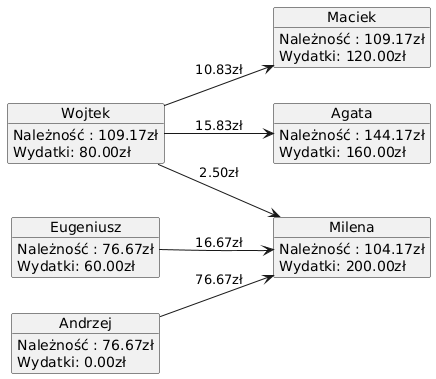
\includegraphics[scale=0.4]{out/diagram_rozliczenie.png}\\\end{document}